
\documentclass[12pt]{article}

% Layout.
\usepackage[top=1.0in, bottom=0.75in, left=1in, right=1in, headheight=1.0in, headsep=0pt]{geometry}

% Fonts.
\usepackage{mathptmx}
\usepackage[scaled=0.86]{helvet}
\renewcommand{\emph}[1]{\textsf{\textbf{#1}}}

% TiKZ.
\usepackage{tikz, pgfplots}
\usetikzlibrary{calc}
\pgfplotsset{my style/.append style={axis x line=middle, axis y line=
middle, xlabel={$x$}, ylabel={$y$}, axis equal }}

% Misc packages.
\usepackage{amsmath,amssymb,latexsym, nicefrac}
\usepackage{graphicx}
\usepackage{array}
\usepackage{xcolor}
\usepackage{multicol}
\usepackage{adjustbox}


% Commands to set various header/footer components.
\makeatletter
\def\doctitle#1{\gdef\@doctitle{#1}}
\doctitle{Use {\tt\textbackslash doctitle\{MY LABEL\}}.}
\def\docdate#1{\gdef\@docdate{#1}}
\docdate{Use {\tt\textbackslash docdate\{MY DATE\}}.}
\def\doccourse#1{\gdef\@doccourse{#1}}
\let\@doccourse\@empty
\def\docscoring#1{\gdef\@docscoring{#1}}
\let\@docscoring\@empty
\def\docversion#1{\gdef\@docversion{#1}}
\let\@docversion\@empty
\makeatother

% Headers and footers layout.
\makeatletter
\usepackage{fancyhdr}
\pagestyle{fancy}
\fancyhf{} % Clears all headers/footers.
\lhead{\emph{\@doctitle\hfill\@docdate}
\ifnum \value{page} > 1\relax\else\\
\emph{Name: \rule{3.5in}{1pt}\hfill \@docscoring}
\\
%\emph{Circle one: \quad Rhodes (F01) \hskip 1ex\rule{1pt}{9pt}\hskip 1ex Bueler (F02)}
\fi}

\rfoot{\emph{\@docversion}}
\lfoot{\emph{\@doccourse}}
\cfoot{\emph{\thepage}}
\renewcommand{\headrulewidth}{0pt}%
\makeatother

% Paragraph spacing
\parindent 0pt
\parskip 6pt plus 1pt

% A problem is a section-like command. Use \problem{5} to
% start a problem worth 5 points.
\newcounter{probcount}
\newcounter{subprobcount}
\setcounter{probcount}{0}
\newcommand{\problem}[1]{%
\par
\addvspace{4pt}%
\setcounter{subprobcount}{0}%
\stepcounter{probcount}%
\makebox[0pt][r]{\emph{\arabic{probcount}.}\hskip1ex}\emph{[#1 points]}\hskip1ex}
\newcommand{\thesubproblem}{\emph{\alph{subprobcount}.}}

% Subproblems are an enumerate-like environment with a consistent
% numbering scheme. 
% Use \begin{subproblems}\item...\item...\end{subproblems}
\newenvironment{subproblems}{%
\begin{enumerate}%
\setcounter{enumi}{\value{subprobcount}}%
\renewcommand{\theenumi}{\emph{\alph{enumi}}}}%
{\setcounter{subprobcount}{\value{enumi}}\end{enumerate}}

% Blanks for answers in normal and math mode.
\newcommand{\blank}[1]{\rule{#1}{0.75pt}}
\newcommand{\mblank}[1]{\underline{\hspace{#1}}}
\def\emptybox(#1,#2){\framebox{\parbox[c][#2]{#1}{\rule{0pt}{0pt}}}}

% Misc.
\renewcommand{\d}{\displaystyle}
\newcommand{\ds}{\displaystyle}
\def\bc{\begin{center}}
\def\ec{\end{center}}

\newcommand{\ans}[1][2]{ \ \rule{#1 in}{.5 pt} \ }


\doctitle{Math 251: Quiz 10}
\docdate{\textbf{Due: Monday Dec 2, 2019}}
\doccourse{UAF Calculus I}
\docversion{v-1}
\docscoring{{\Large \strut}\blank{0.8in} / 25}

\begin{document}
25 points possible.  You may use other sources (books, calculator, friends, etc) but your write up must be your own. The complete quiz is due Monday Dec 2, 2019 at the beginning of class. 

\problem{6} Use Part I of the Fundamental Theorem of Calculus to find the derivative of the function.
\begin{multicols}{2}
	\begin{subproblems}
	\item $g(x)=\d{\int_2^x e^t\cos(t^2) dt}$
	\item $A(x)=\d{\int_{-1}^{x^3}t \ln(3+t^2) dt}$
	\end{subproblems}
\end{multicols}
\vfill
\problem{9} Evaluate each integral below. Assume $a$, $b$, ad $c$ are fixed constants.
	\begin{subproblems}
	\item $\d{\int_{0}^{3} (ax^2-bx+3c)dx}$
	\vfill
	\item $\d{\int_{0}^{\pi/6} \sin(\theta) d\theta}$
	\vfill
	\item $\d{\int_{0}^{4} |x-2| dx }$ (Hint: Interpret as area, sketch a picture, and compute.)
	\vfill
	\end{subproblems}
\problem{4} Let $v(t)$ be the velocity (in meters per second) of a particle moving along a line starting at $t=0.$	
	\begin{subproblems}
	\item What does $\int_1^4 v(t) dt$ represent? 
	\vspace{.4in}
	\item Is it possible for $\int_1^4 v(t) dt$ to be negative? Justify your answer.
	\vspace{.4in}
	\end{subproblems}
	
\newpage	
\problem{3} Find the \emph{exact} value of the area shaded below. Show your work. \\
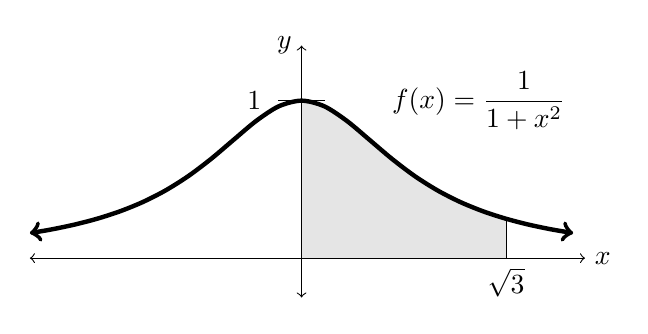
\begin{tikzpicture}[xscale = 1.5,yscale=2]
%shade part
\fill [gray!20, domain=0:1.732, variable=\x]
  (0, 0)
  -- plot ({\x}, {1/(1+\x*\x})
  -- (1.732, 0)
  -- cycle;
 %curve
  \draw[ultra thick, <->] plot[smooth, domain=-2.3:2.3]({\x,1/(1+\x*\x)});
 
\draw (1.732, 1/4)--(1.732,0) node[below] {$\sqrt{3}$};
\draw[<->] (-2.3,0) -- (2.4,0) node[right]{$x$};
\draw[<->] (0,-.25) -- (0, 1.35) node[left]{$y$};;
%\draw (.1, 1/2)-- (-.1, 1/2) node[left]{{\small $\nicefrac{1}{2}$}} ;
%\draw (.1, 1/4)-- (-.1, 1/4) node[left]{{\small $\nicefrac{1}{4}$}} ;
%\draw (.1, 3/4)-- (-.1, 3/4) node[left]{{\small $\nicefrac{3}{4}$}} ;
\draw (.2, 1)-- (-.2, 1) {} ;
\node at (-.4,1){1};
\node at (1.5,1){$f(x)=\d{\frac{1}{1+x^2}}$};

\end{tikzpicture}

\vspace{2in}
\problem{3} Let $Q(x) = \d{\int_{0}^x P(t) dt}$, where $P(t)$ is the function whose graph is shown below.\\

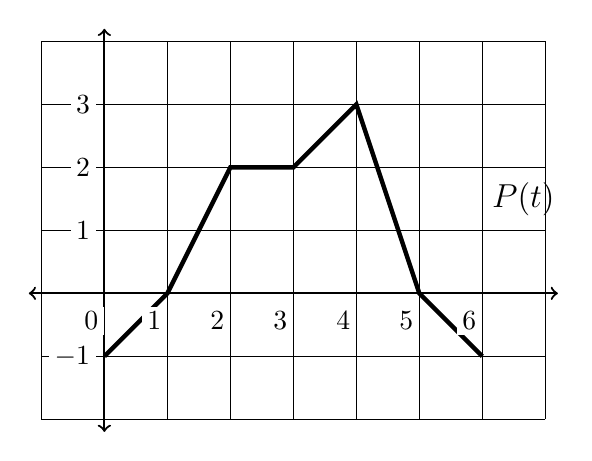
\begin{tikzpicture}[scale=.8]
\draw[thin] (-1,-2) grid (7,4);
\draw[<->, thick] (-1.2,0) -- (7.2,0);
\draw[<->, thick] (0,-2.2) -- (0, 4.2);
\draw[ultra thick] (0,-1) --(1,0)-- (2,2) -- (3,2) -- (4,3) -- (5,0) -- (6,-1);
\foreach \i in {-1,1,2,3}{\draw (0,\i) node[left=3 pt,fill=white, inner sep=2pt] {$\i$};}
\foreach \i in {0,1,2, 3,4,5,6}{\draw (\i,0) node[below=10pt, left= .01 pt, fill=white, inner sep=2pt] {$\i$};}
\draw (6,1.5) node[right]{\large{$P(t)$}}; 
\end{tikzpicture}


	\begin{subproblems}
	\item Find $Q(2)$
	\vfill
	\item On what interval is $Q(x)$ increasing?
	\vfill
	\item Where does $Q(x)$ have a maximum?
	\vfill
	\end{subproblems}
\end{document}

